% ----------------------------------------------------
% -------- BAYSIS - Selected as Jam Follower ---------
% ----------------------------------------------------
\subsection{Accident - Selected as Jam Follower}
\label{analysis_processing_correlation_baysis_follower}
The correlation matrix table for the congestion-accident \textit{Jam Follower} dataset (see \cref{table:appendix_correlation_matrix_matched_cramers}) is visual presented in \cref{img:correlation_matrix_selected_effector_cramers} showing the the correlation of each variable combination. When visual analyzing \cref{img:correlation_matrix_matched_cramers} and checking the guidelines for a strong correlation in reference to the applied coefficient (identifiable with \cref{table:appendix_coefficient_matrix_matched}) we get a list of strongly correlated variable combinations (see \cref{tbl:correlation_list_baysis_follower}). Since the focus of the thesis are the correlations between accidents and jams, these are only collected from the bottom-left rectangle of the matrix, where the congestion and accidents variables intersect.

\noindent
\begin{table}[h!]
	\centering
	\begin{tabular}{c|l}  
		Category & Strong \\
		\\[-1em]
		\hline
		\\[-1em]
		Strasse & TMax, TAvg, SMax, SAvg, TDist, SDist, Cov, TLHGV \\ 
 		Kat & TMax, SAvg \\ % + SMax % -> Strasse
 		%Typ & \\ + Cov % -> Strasse
 		%Betei & \\ % -> Strasse
 		UArt1 & TAvg, SAvg, TDist, Cov, TLHVG \\ % + SMax % -> Strasse
 		UArt2 & TDist \\ % + Cov % -> Strasse
 		AUrs1 & TDist, SDist, Cov, TLHGV \\ % -> Strasse
 		%AUrs2 & \\ % -> Strasse
 		AufHi & TMax, TAvg, Cov \\ % -> Strasse
 		%Alkoh & \\
 		%Char1 & \\ % -> Strasse
 		%Char2 & \\ % -> Strasse
 		Lich1 & Cov \\ % -> Strasse
 		%Lich2 & \\ + Cov % -> Strasse
 		%Zust1 & \\ + Cov % -> Strasse
 		%Zust2 & \\ % -> Strasse
 		%Fstf & \\ % -> Strasse
 		WoTag & TAvg, SMax, SAvg, TDist, Cov, TLHGV \\ % + TLCar % -> Strasse
 		%FeiTag & \\
 		Month & TMax, TAvg, SMax, Cov, TLHGV \\ % + SAvg % -> Strasse
	\end{tabular}
    \caption{List of incident variables and their strong correlated congestion variable from the congestion-accident matched data which are classified as \textit{Jam Follower}}
	\label{tbl:correlation_list_baysis_follower}
\end{table}

Next we need to verify that the correlation is significant and what the correlation predicates. Therefore each correlation will be evaluated with the Post Hoc test, defined in \cref{correlation_posthoc}. In the following sections, the correlated relations of the variables in \cref{tbl:correlation_list_baysis_follower} are analyzed and an initial interpretation of each significant correlation is introduced. Groups with an insufficient sample size (see \cref{correlation_uncertainty} are neglected and not shown. The descriptive tables, showing the count ($n$), mean ($\bar{x}$), standard deviation ($\sigma$), median ($\tilde{x}$), $min$, $max$ and range ($\Delta$) therefore only contain groups with significant sample sizes.

\begin{figure}[!ht]
	\centering
	\makebox[\textwidth][c]{%
		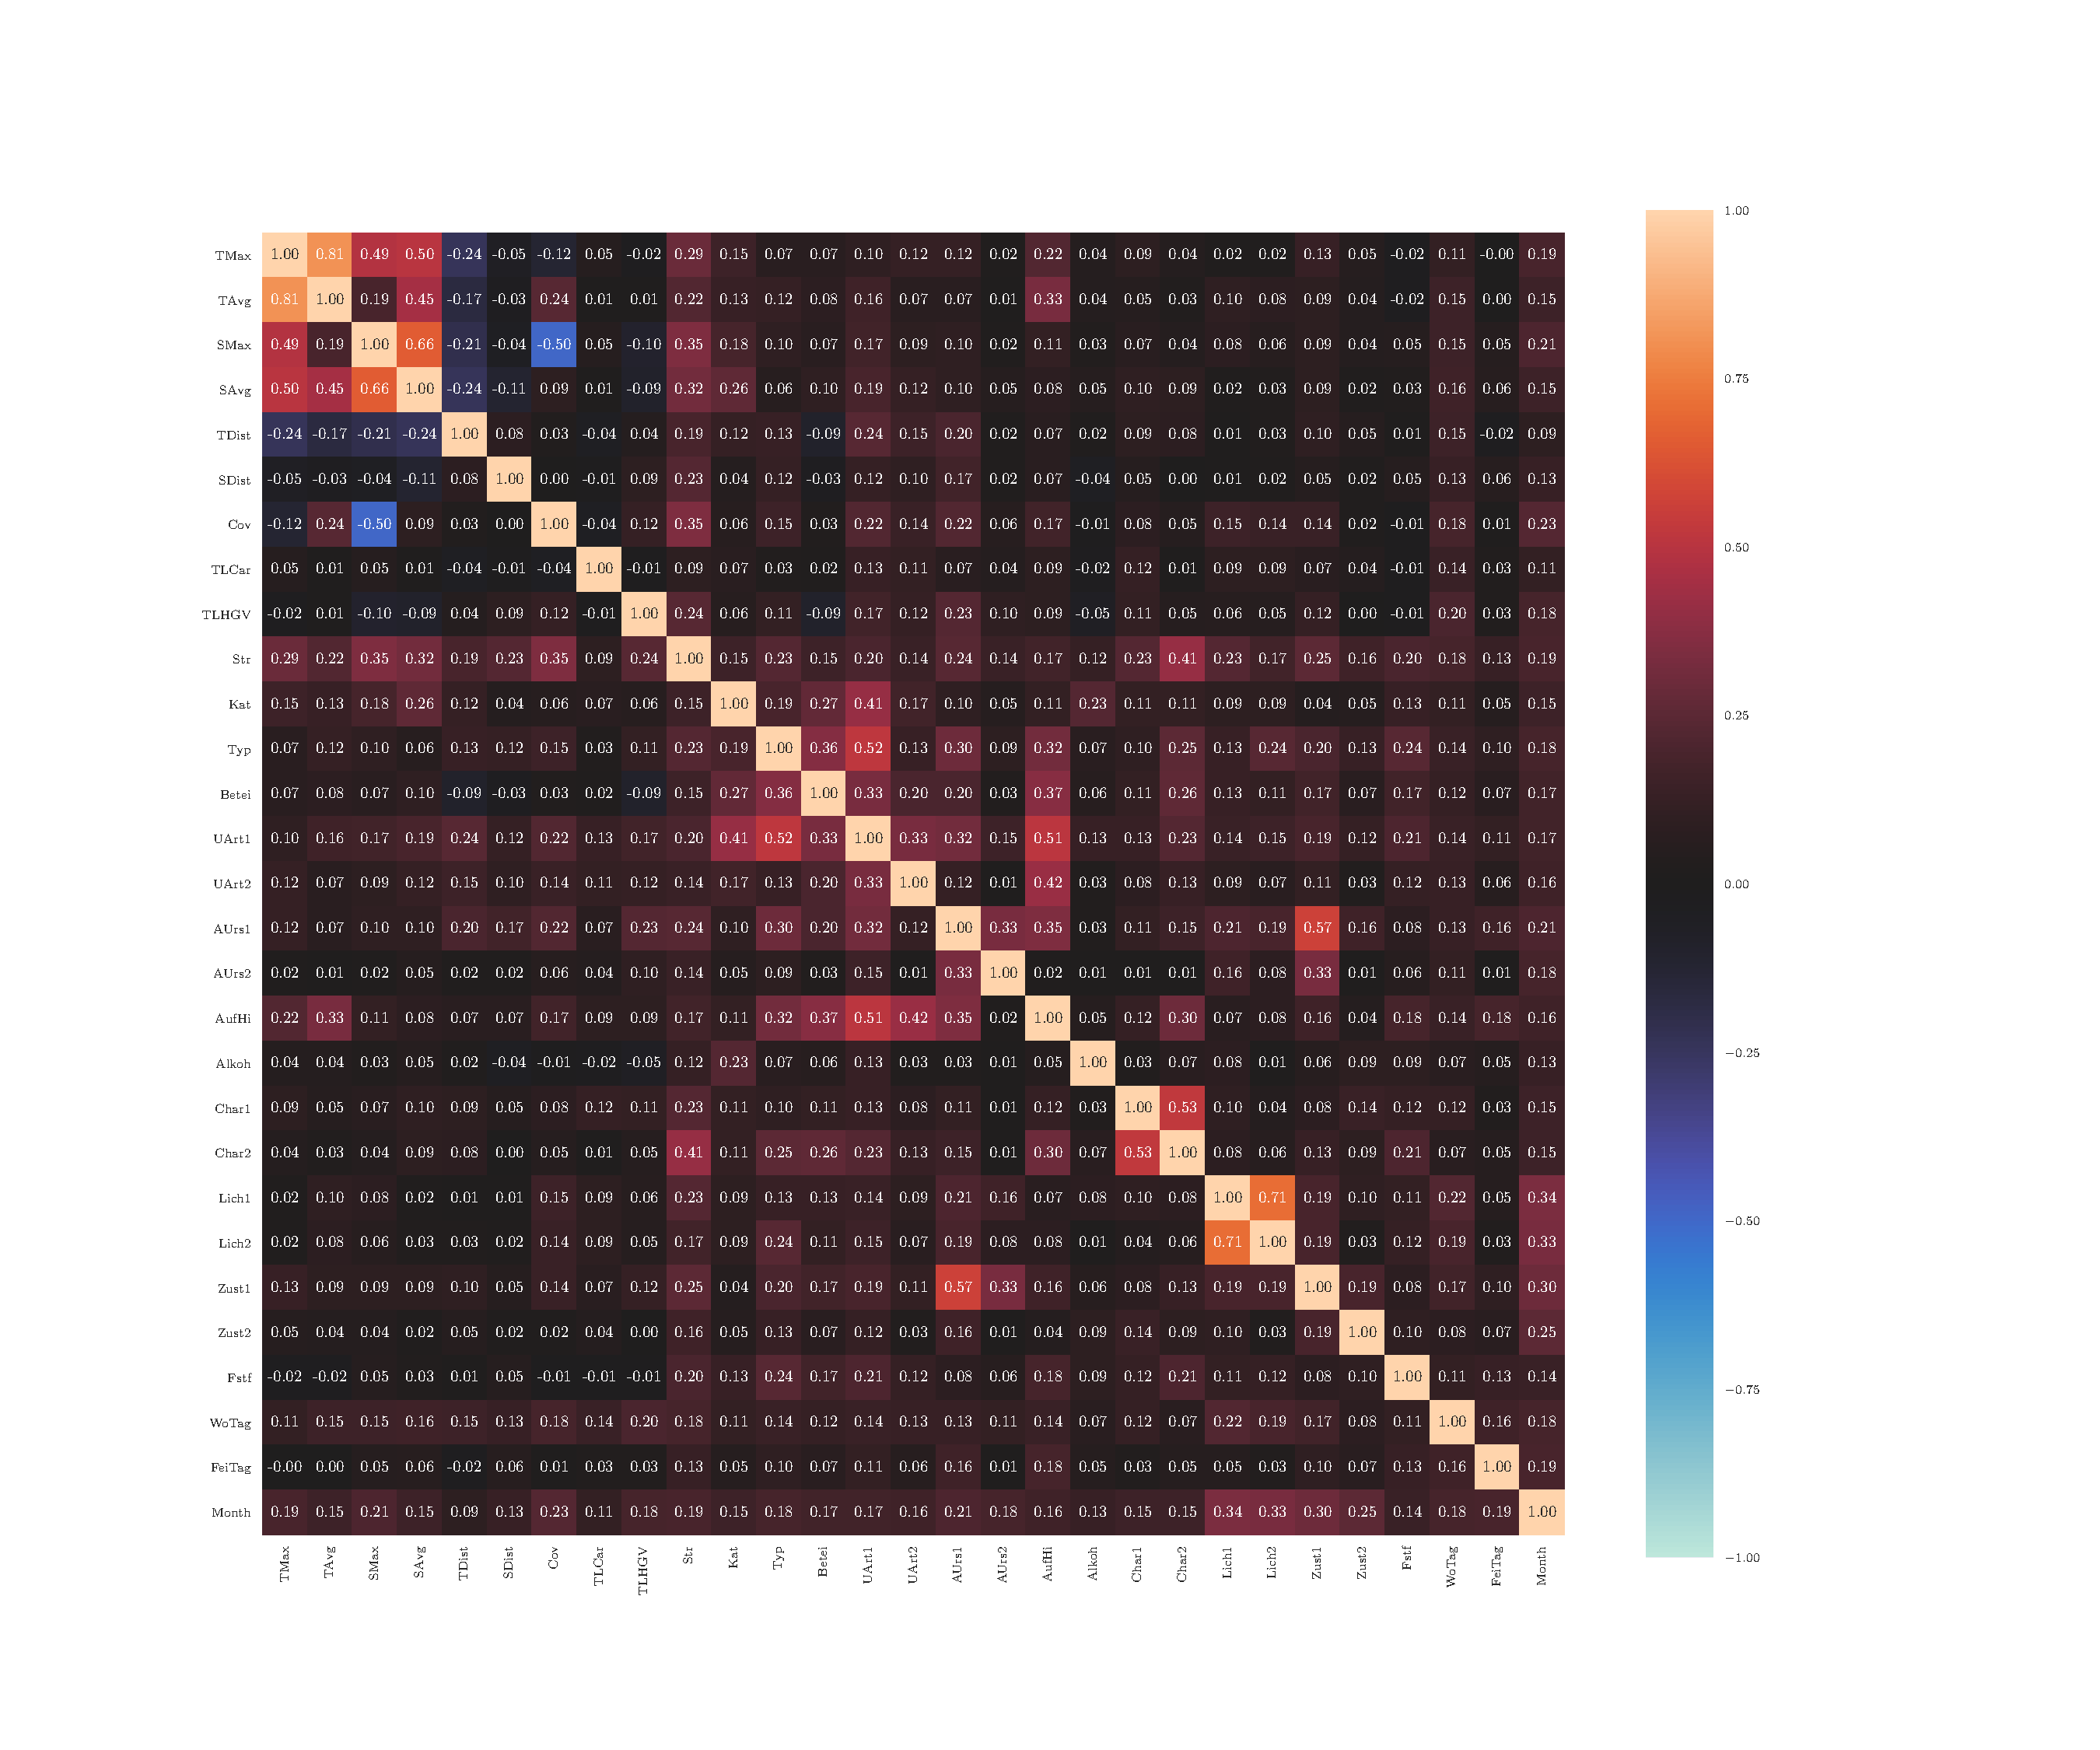
\includegraphics[width=1.4\textwidth, trim=0cm 2.5cm 6cm 3cm]{CorrAnalysis/data/BAYSIS/03_selected_03_endJam/plots/baysis_selected_corr_cramers}%
	}
	\caption{Correlation matrix for congestion-accident matched data classified as \textit{Jam Effector}, with $V$, $\eta$, $\tau$, $r_{pq}$, $r$}
	\label{img:correlation_matrix_selected_effector_cramers}
\end{figure}

% --------------------------
% -------- Strasse ---------
% --------------------------
\centerheading{Strasse}
All relations of \textit{Strasse} - \textit{TMax}, \textit{Strasse} - \textit{TAvg}, \textit{Strasse} - \textit{SMax}, \textit{Strasse} - \textit{SAvg}, \textit{Strasse} - \textit{TDist}, \textit{Strasse} - \textit{SDist}, \textit{Strasse} - \textit{Cov} and \textit{Strasse} - \textit{TLHGV} produce a $p$-value above the $\alpha$-level. The null hypothesizes can't be rejected and there are no significant differences in the variable \textit{Strasse} in these relations.

% ----------------------
% -------- Kat ---------
% ----------------------
\centerheading{Kat}
Both relations of \textit{Kat} - \textit{TMax} and \textit{Kat} - \textit{SAvg} produce a $p$-value above the $\alpha$-level. The null hypothesizes can't be rejected and there are no significant differences in the variable \textit{Kat} in these relations.

% ------------------------
% -------- UArt ---------
% ------------------------
\centerheading{UArt}
All relations of \textit{UArt1} - \textit{TAvg}, \textit{UArt1} - \textit{SAvg}, \textit{UArt1} - \textit{TDist}, \textit{UArt1} - \textit{Cov}, \textit{UArt1} - \textit{TLHGV} and \textit{UArt2} - \textit{TDist} produce a $p$-value above the $\alpha$-level. The null hypothesizes can't be rejected and there are no significant differences in the variable \textit{Strasse} in these relations.

% ------------------------
% -------- AUrs ---------
% ------------------------
\centerheading{AUrs}
This section analyzes the correlated relations of the accident variable \textit{AUrs1}. The correlations of \textit{AUrs1} - \textit{TDist} and \textit{AUrs1} - \textit{TLHGV} produces a $p$-value above the $\alpha$-level of .05 in the Kruskal-Wallis rank sum test. The null hypothesis can't therefore be rejected for these relations and there are no significant groups to identify.

The Kruskal-Wallis rank sum test of \textit{AUrs1} - \textit{SDist} produces a $p$-value of 0.0372, which is below $\alpha=.05$. The null hypothesis can therefore be rejected, which means there is a significant difference in the variable \textit{Strasse}. To identify the significant groups, a pairwise Wilcoxon $T$-test for \textit{AUrs1} - \textit{TMax} is run, which produces \cref{tbl:wilcoxon_baysis_follower_AUrs1_SDist}. 
\begin{table}[ht]
	\tiny
	\centering
	\begin{tabular}{rrrrrrr}
		\toprule
		& 0 & 72 & 73 & 80 & 82 & 88 \\ 
		\midrule
		72 & 1.00 &  &  &  &  &  \\ 
		73 & 0.10 & 0.35 &  &  &  &  \\ 
		80 & 1.00 &  & 1.00 &  &  &  \\ 
		82 & 1.00 &  & 1.00 &  &  &  \\ 
		88 & 0.40 & 0.04 & 1.00 & 1.00 & 0.55 &  \\ 
		89 & 1.00 &  & 1.00 &  &  & 1.00 \\ 
		\bottomrule
	  \end{tabular}
    \caption{Pairwise Wilcoxon $T$-test for \textit{AUrs1} and \textit{Spatial Distance} (Jam Follower)}
    \label{tbl:wilcoxon_baysis_follower_AUrs1_SDist}
\end{table}
The tables shows that the differences are not group specific, which means that the relation can be neglected (see \cref{correlation_posthoc}).

The Kruskal-Wallis rank sum test of \textit{AUrs1} - \textit{Cov} produces a $p$-value of 0.0024, which is below $\alpha=.05$. The null hypothesis can therefore be rejected, which means there is a significant difference in the variable \textit{Strasse}. To identify the significant groups, a pairwise Wilcoxon $T$-test for \textit{AUrs1} - \textit{Cov} is run, which produces \cref{tbl:wilcoxon_baysis_follower_AUrs1_Cov}. 
\begin{table}[ht]
	\tiny
	\centering
	\begin{tabular}{rrrrrrr}
		\toprule
		& 0 & 72 & 73 & 80 & 82 & 88 \\ 
		\midrule
		72 & 0.28 &  &  &  &  &  \\ 
		73 & 1.00 & 1.00 &  &  &  &  \\ 
		80 & 1.00 & 1.00 & 1.00 &  &  &  \\ 
		82 & 1.00 & 1.00 & 1.00 & 1.00 &  &  \\ 
		88 & 0.33 & 0.79 & 0.56 & 1.00 & 1.00 &  \\ 
		89 & 1.00 & 1.00 & 1.00 & 1.00 & 1.00 & 1.00 \\ 
		\bottomrule
	  \end{tabular}
    \caption{Pairwise Wilcoxon $T$-test for \textit{AUrs1} and \textit{Coverage} (Jam Follower)}
    \label{tbl:wilcoxon_baysis_follower_AUrs1_Cov}
\end{table}
The tables shows that the differences are not group specific, which means that the relation can be neglected (see \cref{correlation_posthoc}).

% ------------------------
% -------- AufHi ---------
% ------------------------
\centerheading{AufHi}
All relations of \textit{AufHi} - \textit{TMax}, \textit{AufHi} - \textit{TAvg} and \textit{AufHi} - \textit{Cov} produce a $p$-value above the $\alpha$-level. The null hypothesizes can't be rejected and there are no significant differences in the variable \textit{AufHi} in these relations.

% ------------------------
% -------- Lich1 ---------
% ------------------------
\centerheading{Lich}
The relation of \textit{Lich1} - \textit{Cov} produce a $p$-value above $\alpha=.05$ in the Kruskal-Wallis rank sum test. The null hypothesizes can't be rejected and there are no significant differences in the variable \textit{Lich1}.

% ------------------------
% -------- WoTag ---------
% ------------------------
\centerheading{WoTag}
All relations of \textit{WoTag} - \textit{TMax}, \textit{WoTag} - \textit{SMax}, \textit{WoTag} - \textit{SAvg}, \textit{WoTag} - \textit{TDist}, \textit{WoTag} - \textit{Cov} and \textit{WoTag} - \textit{TLHGV} produce a $p$-value above the $\alpha$-level. The null hypothesizes can't be rejected and there are no significant differences in the variable \textit{WoTag} in these relations.

% ------------------------
% -------- Month ---------
% ------------------------
\centerheading{Month}
All relations of \textit{Month} - \textit{TMax}, \textit{Month} - \textit{SMax}, \textit{Month} - \textit{SAvg}, \textit{Month} - \textit{Cov} and \textit{Month} - \textit{TLHGV} produce a $p$-value above the $\alpha$-level. The null hypothesizes can't be rejected and there are no significant differences in the variable \textit{Month} in these relations.